\chapter{Diseño del editor}

En este capítulo nos centraremos en los detalles concretos del diseño del editor. El editor resultante se compone de tres módulos bien diferenciados que son son el núcleo del editor, el editor de fórmulas y el purificador de HTML.

El núcleo del editor es un fichero Javascript que será el responsable de llevar a cabo la mayor parte de las funciones del editor. Este fichero encapsula la funcionalidad de la aplicación en la clase SwadeManager, SwadeDialog y SwadePanel. La primera de ella es una clase donde todos los métodos son estáticos y usamos para las distintas operaciones que componen la funcionalidad del editor. 

SwadeDialog es una clase que nos permite crear Dialog propios como el de la figura ~\ref{fig:dialog} y ofrece principalmente métodos para mostrarlos, ocultarlos y destruirlos.


\begin{figure}[h!]
  \centering
      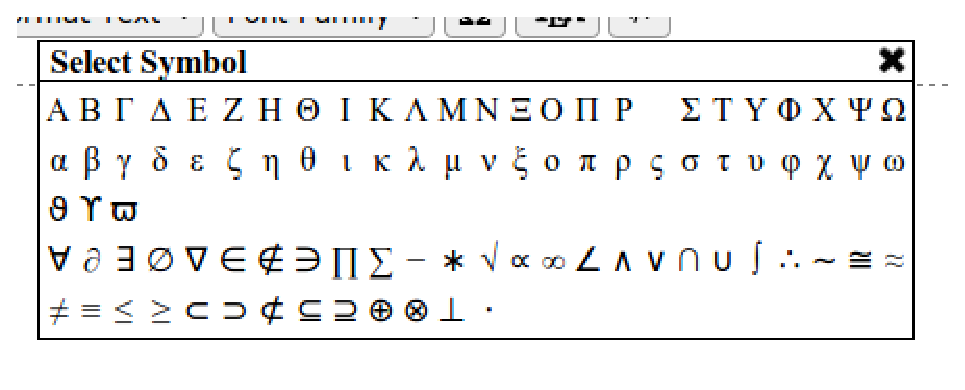
\includegraphics[width=4in]{fig/dialog}
  \caption{Dialogo creado con SwadeDialog.}
  \label{fig:dialog}

\end{figure}


SwadePanel es la clase que encapsula los métodos propios de cada editor. Estos métodos son principalmente para bloquear un editor cuando no se ha seleccionado y para el refresco del formato del texto seleccionado ~\ref{fig:panel}.

\begin{figure}[h!]
  \centering
      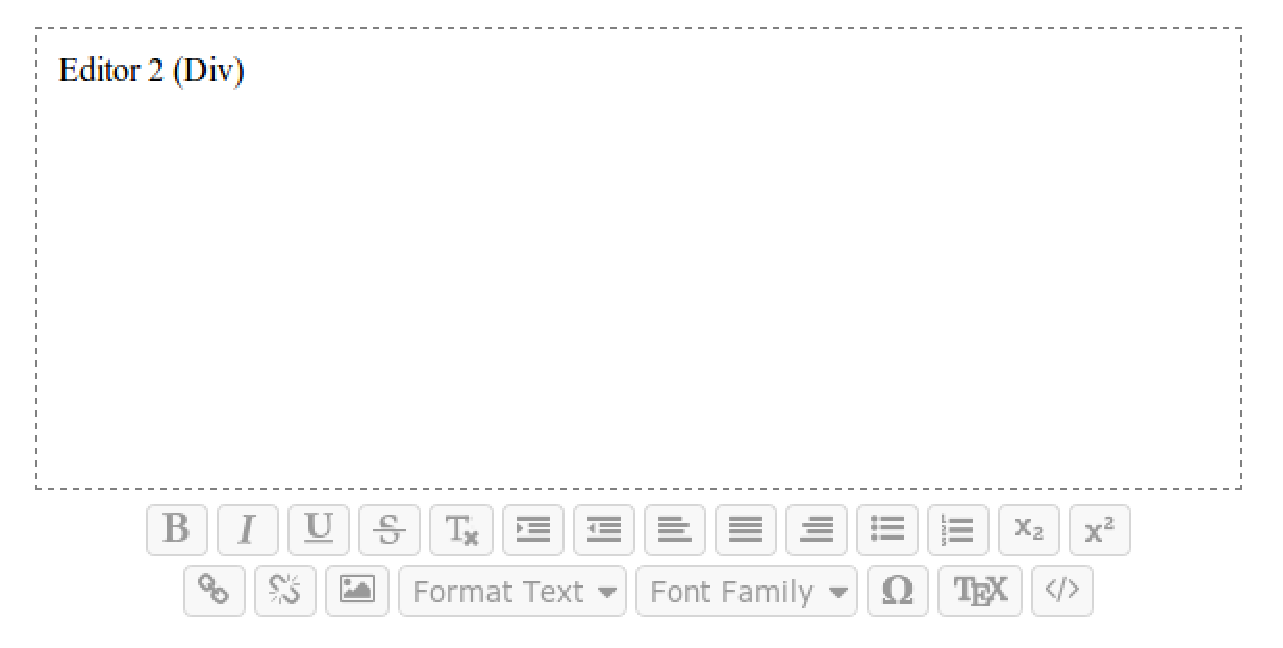
\includegraphics[width=7in]{fig/panel}
  \caption{Editor SWADE bloqueado.}
  \label{fig:panel}

\end{figure}


Para usar SWADE debemos incluir el fichero javascript con el código siguiente.

\begin{verbatim}
<script src="path-to-swade/swade.js" type="text/javascript"></script>
\end{verbatim}

Este script convierte uno o varios textarea o div en un editor SWADE. Para instanciar un editor en un textarea o div tenemos tres métodos. Por id, por clase o realizando una consulta. En el fragmento de código siguiente vemos un ejemplo de cada uno de ellos.

\begin{verbatim}
<script>
  SwadeManager.setOnDOMLoaded(function(){
  SwadeManager.setSwadeByQuery("textarea.swade"); //1
  SwadeManager.setSwadeById("swade-id");          //2
  SwadeManager.setSwadeByClassName("swade-class");//3
  }
  );
</script>
\end{verbatim}
La función SwadeManager.setOnDOMLoaded aplica la función pasada por parámetro cuando se ha construido completamente lo que se conoce por Document Object Model, aunque las imágenes aún estén en carga.
A esta función le pasaremos los métodos para instanciar el editor en las distintas partes de la página. Con el primero de ellos instanciaremos un editor en aquellos textarea con la clase ``swade'', con el segundo lo haremos para los elementos div o textarea con id ``swade-id'' y con el último instanciaremos el editor para los elementos div o textarea con clase ``swade-class''. 

Todas estas funciones se apoyan en las distintas funciones de selección de Javascript y la función setSwade, que instancia un editor para cada elemento de un vector de elementos. En esta función se tiene en cuenta si el objetivo es un div o un textarea, siendo este último el caso más complejo. Si el objetivo es un div se añade a este un panel al que añadimos los distintos eventos de pulsación de los distintos botones. Por el contrario, si el objetivo es un textarea, debemos crear nosotros mismo el elemento div, asignarle como contenido el valor del textarea, ocultar dicho textarea y comprobar si formaba parte de un formulario. Si el textarea formaba parte de un formulario, debemos interceptar la petición del formulario para establecer el valor del textarea al valor del div que estamos editando. 


El editor de fórmulas es una página HTML que usa la herramienta Mathjax para renderizar la fórmula en tiempo real usando HTML y CSS. Este proceso se lleva a cabo mientras que el usuario la escribe dicha fórmula. 

Cuando el usuario finaliza la inserción de la fórmula, enviamos una petición asíncrona al servidor al script tex2png.php que nos devolverá el elemento HTML correspondiente a la imagen generada. El fragmento de código siguiente es el responsable de hacer la petición al servidor de forma asíncrona, de insertar la imagen devuelta por este en SWADE y de cerrar la ventana del editor de fórmulas. 

\begin{verbatim}

function showFormula(str)
{
    var xmlhttp;
    if (window.XMLHttpRequest)
    {// code for IE7+, Firefox, Chrome, Opera, Safari
        xmlhttp=new XMLHttpRequest();
    }
    else
    {// code for IE6, IE5
        xmlhttp=new ActiveXObject("Microsoft.XMLHTTP");
    }
    xmlhttp.onreadystatechange=function()
    {
        if (xmlhttp.readyState==4 && xmlhttp.status==200)
        {
            opener.tex = xmlhttp.responseText;
            window.returnValue = xmlhttp.responseText;
            top.close();
            return false;
        }
    }
    xmlhttp.open("POST","tex2png.php",true);
    xmlhttp.setRequestHeader("Content-type","application/x-www-form-urlencoded");
    xmlhttp.send("MathInput="+encodeURIComponent(str));

}

\end{verbatim}

Para el editor de fórmulas, en la parte del servidor, encontramos el script tex2png.php (que no tiene nada que ver con la herramienta tex2png descrita en el capítulo \emph{Estado del arte}).

Este script se ocupa de extraer el valor de la fórmula de la variable POST, de generar la imagen correspondiente con texvc y de devolver el elemento HTML necesario para insertar dicha fórmula en nuestro editor SWADE. El fragmento de código siguiente recoge dicha funcionalidad.

\begin{verbatim}
...
$latex_formula = "'".$_POST["MathInput"]."'";
$cadena = "./texvc $path_tmp $path_dest $latex_formula";
exec($cadena,$output,$return);
...
echo "<img src=\"${cwd}/${path_dest}${name}.png\" alt=\"Formula inválida\" 
data-tex-swade = $latex_formula 
onclick=\"swade_app.tex_code_selected = $latex_formula;\
swade_app.selected_tex_object = this;\" 
style=\"vertical-align:middle;\"/>";
\end{verbatim}

Podemos observar como se han añadido algunos atributos al elemento HTML para insertar la imagen, aparte de la ruta de esta. El atributo data-tex-swade y onclick son para poder editar la fórmula haciendo click sobre ella. El atributo style es para alinear la fórmula con el texto que la rodea.


El último modulo de nuestro editor es la herramienta HTMLpurifier~\cite{htmlpurifier}, la cual se ocupará del filtrado del HTML generado por el usuario. Dicha herramienta está escrita en php y nos permitirá evitar ataques XSS en la página de la plataforma. En el siguiente fragmento de código se muestra un ejemplo de uso de dicha herramienta.

\begin{verbatim}
...
require_once '../htmlpurifier/library/HTMLPurifier.auto.php';
$config = HTMLPurifier_Config::createDefault();
$config->set('Core.Encoding', 'UTF-8'); 
$config->set('HTML.Doctype', 'HTML 4.01 Transitional'); 
$purifier = new HTMLPurifier($config);
...
$parsed_content = $purifier->purify($_POST['editor3']);
...
\end{verbatim}

Para usar dicha herramienta debemos instanciar el purificador con una configuración determinada y finalmente aplicar el método purify sobre el texto que queremos purificar. Dado que la plataforma usa la codificación ISO-8859-1, en este punto tendremos que tener en mente una serie de consideraciones recogidas en el apéndice \emph{Integración en la plataforma SWAD}.

